\section{Trả lời câu hỏi}
\subsection{Câu 1}
\textbf{Câu hỏi: Một số cảm biến dòng điện trên thị trường}

\begin{enumerate}
    \item \textbf{TMCS1101}: dùng rộng rãi từ đo dòng nhỏ trong hệ thống điện tử đến đo dòng lớn hơn trong thiết bị công nghiệp. Cảm biến này sử dụng hiệu ứng Hall để đo dòng trực tiếp từ từ trường.
    \begin{itemize}
        \item \textbf{Dòng tối đa}: Phụ thuộc vào phiên bản: ±20A, ±50A, ±100A lần lượt ứng với TMCS1101A1, TMCS1101A2 và TMCS1101A3.
        \item \textbf{Cách lấy giá trị}: Đầu ra dạng analog, đọc qua ADC.
        \item \textbf{Nguồn tham khảo}: \href{https://www.ti.com/product/TMCS1101}{Texas Instruments - TMCS1101}.
        \item \textbf{Hình ảnh}:
        \begin{center}
            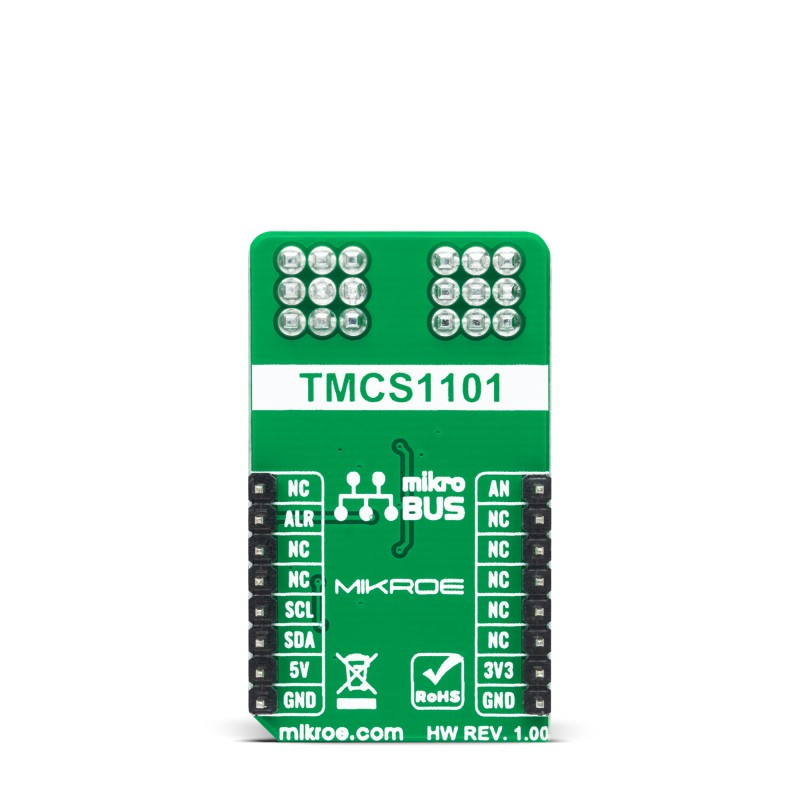
\includegraphics[width=0.2\textwidth]{graphics/section5/tmcs1101.png}
        \end{center}
    \end{itemize}

    \item \textbf{INA226}:
    \begin{itemize}
        \item \textbf{Dòng tối đa}: Cảm biến này đo dòng điện thông qua điện áp trên điện trở Shunt. Dòng đo được tối đa phụ thuộc vào giá trị điện trở, chỉ biết ngưỡng điện áp đầu vào là ±36V.
        \item \textbf{Cách lấy giá trị}: Giao tiếp I2C.
        \item \textbf{Nguồn tham khảo}: \href{https://www.ti.com/product/INA226}{TI - INA226}.
        \item \textbf{Hình ảnh}:
        \begin{center}
            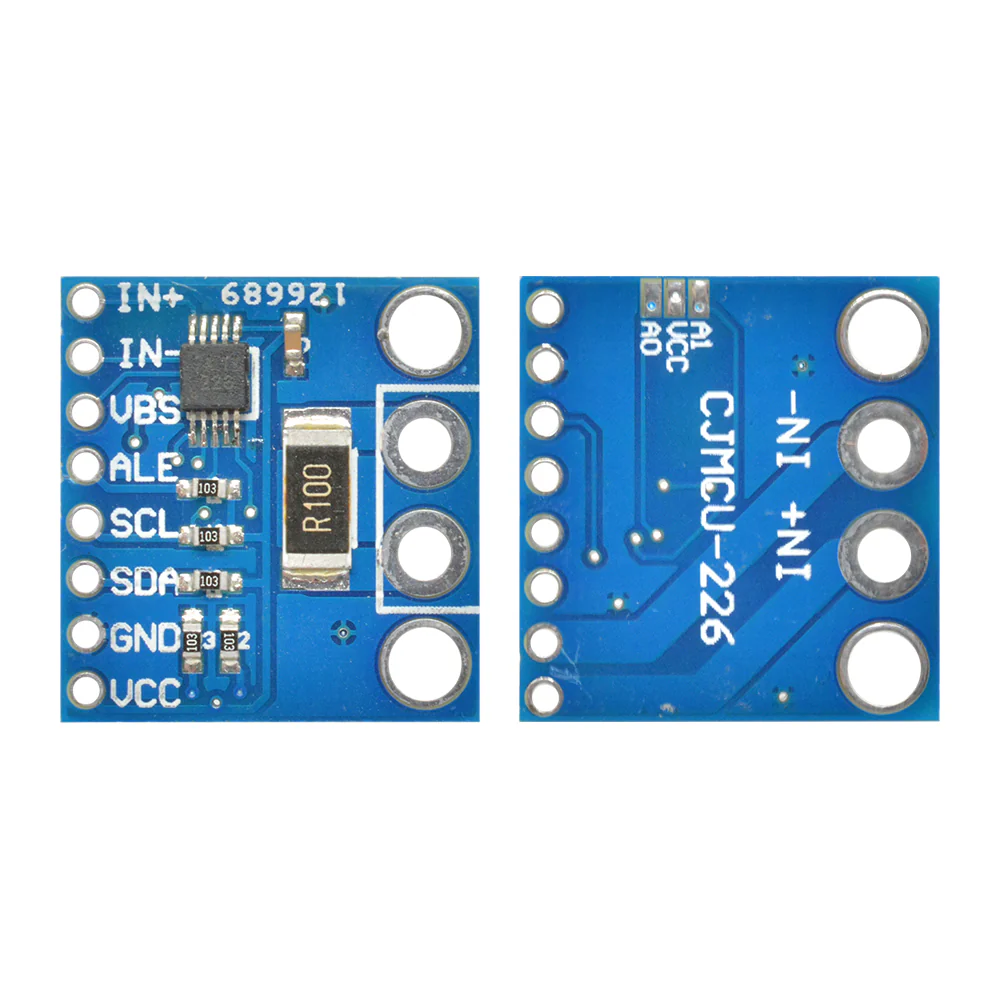
\includegraphics[width=0.3\textwidth]{graphics/section5/ina226.png}
        \end{center}
    \end{itemize}

    \item \textbf{LTC2945}:
    \begin{itemize}
        \item \textbf{Dòng tối đa}: Cảm biến này đo dòng điện thông qua điện áp trên điện trở Shunt. Giá trị dòng điện tối đa phụ thuộc giá trị điện trở. Ngưỡng điện áp đầu vào: $4V - 80V$.
        \item \textbf{Cách lấy giá trị}: Giao tiếp I2C hoặc SMBus.
        \item \textbf{Nguồn tham khảo}: \href{https://www.analog.com/en/products/ltc2945.html}{Analog Devices - LTC2945 Datasheet and Product Info}.
        \item \textbf{Hình ảnh}:
        \begin{center}
            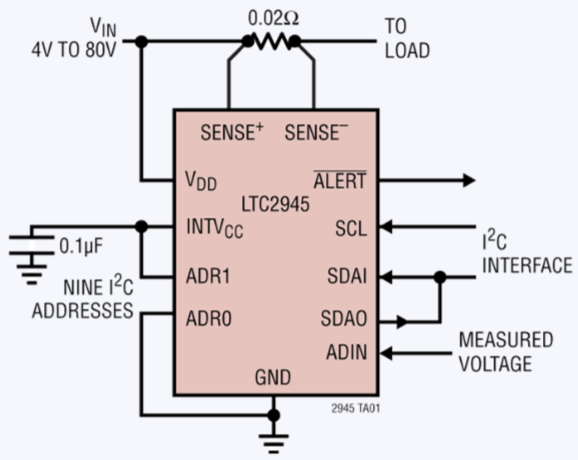
\includegraphics[width=0.6\textwidth]{graphics/section5/ltc2945.png}
        \end{center}
    \end{itemize}

    \item \textbf{LEM HXS 20-NP}:
    \begin{itemize}
        \item \textbf{Dòng tối đa}: ±20A. Cảm biến này đo dòng điện trực tiếp thông qua từ trường, dựa vào nguyên lý Hall.
        \item \textbf{Cách lấy giá trị}: Đầu ra dạng analog, đọc qua ADC.
        \item \textbf{Nguồn tham khảo}: \href{https://www.lem.com/sites/default/files/products_datasheets/hxs_20-np.pdf}{LEM - HXS 20-NP Datasheet}.
        \item \textbf{Hình ảnh}:
        \begin{center}
            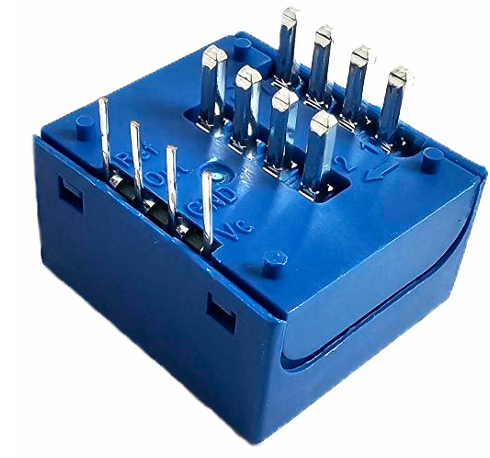
\includegraphics[width=0.4\textwidth]{graphics/section5/lem_hxs20np.png}
        \end{center}
    \end{itemize}

    \item \textbf{WCS1800}:
    \begin{itemize}
        \item \textbf{Dòng tối đa}: ±35A với dòng DC và ±25A với dòng AC. Cảm biến này đo dòng điện trực tiếp thông qua từ trường, dựa vào nguyên lý Hall.
        \item \textbf{Cách lấy giá trị}: Đầu ra dạng analog, đọc qua ADC.
        \item \textbf{Nguồn tham khảo}: \href{https://www.winson.com.tw/uploads/images/WCS1800.pdf}{Winson Electronics - WCS1800}.
        \item \textbf{Hình ảnh}:
        \begin{center}
            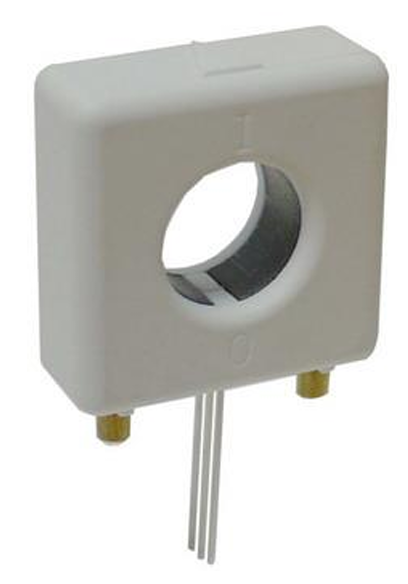
\includegraphics[width=0.4\textwidth]{graphics/section5/wcs1800.png}
        \end{center}
    \end{itemize}

\end{enumerate}
\pagebreak
\subsection{Câu 2}
\textbf{Câu hỏi: Trong \ref{subsec: Interfacing Slide Switch with an MCU}, điện áp của SW1 khi công tắc trượt 1 bật và khi tắt là bao nhiêu?}

\textbf{Trả lời}
\begin{itemize}
    \item Khi công tắc trượt 1 bật, SW1 được nối với GND nên điện áp tại SW1 bằng 0V.
    \item Khi công tắt trượt 1 tắt, mạch hở tại GND nên không có dòng điện chạy qua trở (hoặc rất nhỏ). Ta có $V_{SW1} = V_{3.3V} - I.R = V_{3.3V}$, do đó điện áp tại SW1 là 3.3 V 
\end{itemize}

\textbf{Mô phỏng}

Trong mạch \ref{subsec: Interfacing Slide Switch with an MCU}, các SW được nối vào chân GPIO của ESP32-WROM-32 part nên ta mô phỏng SW sẽ được nối theo kiểu chân đầu ra GPIO push-pull.

\begin{figure}[ht]
    \centering
    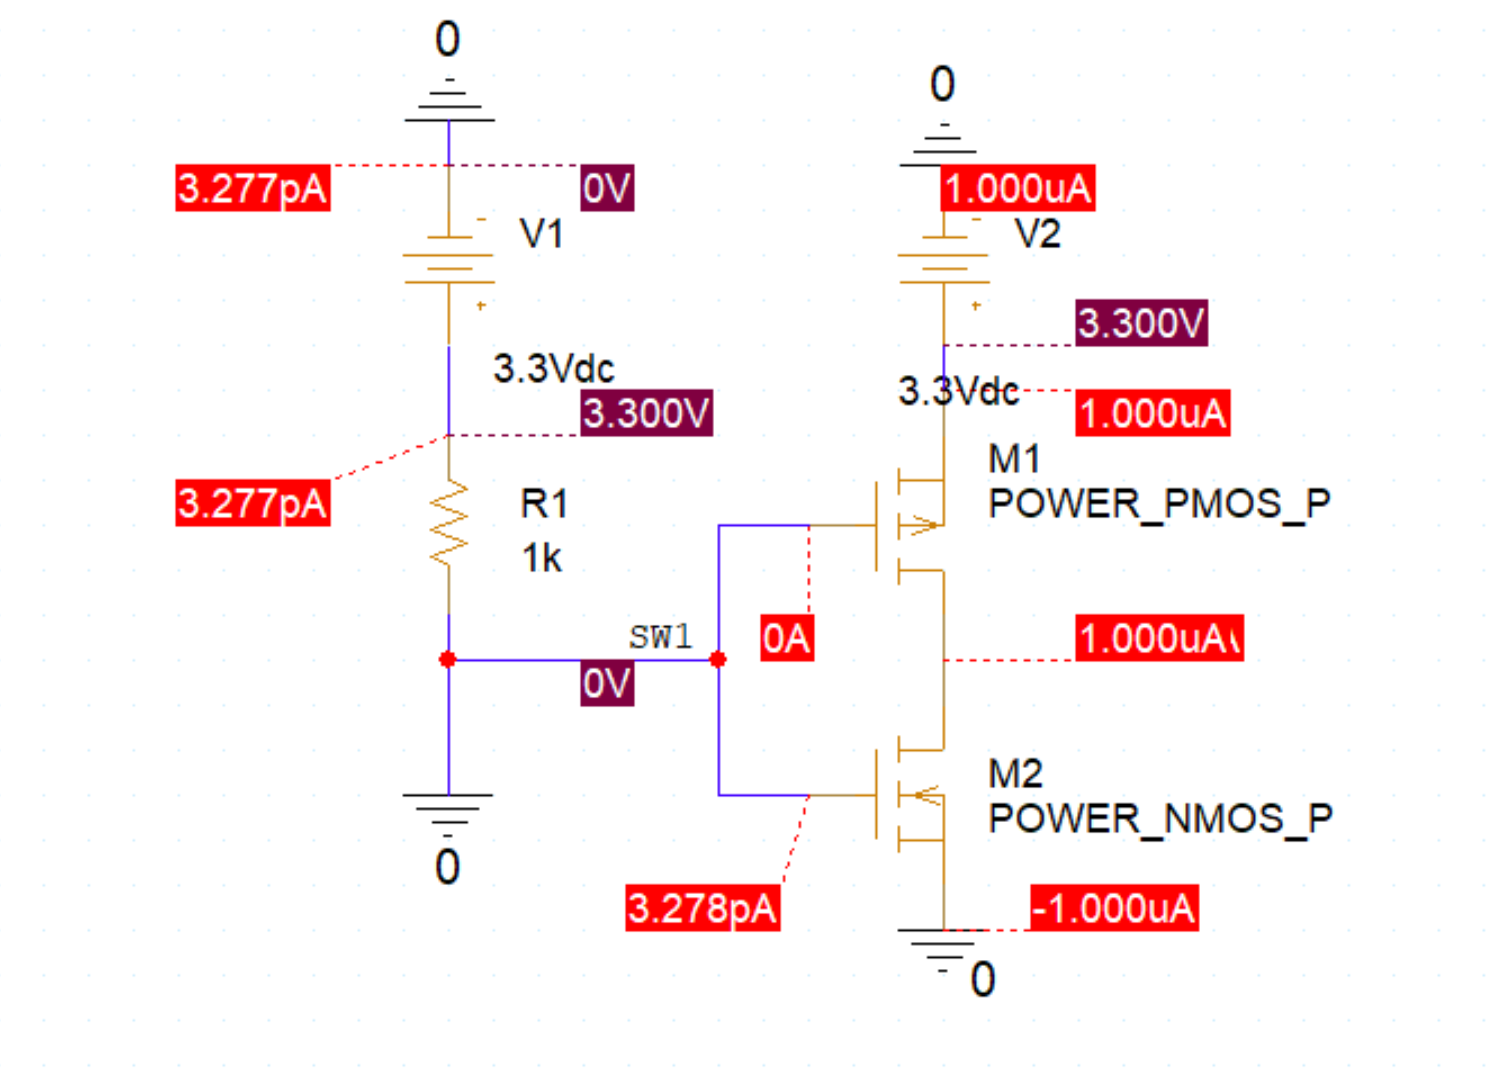
\includegraphics[width=0.7\textwidth]{graphics/section5/f1.png}
    \caption{SW1 ON}
\end{figure}

\begin{figure}[ht]
    \centering
    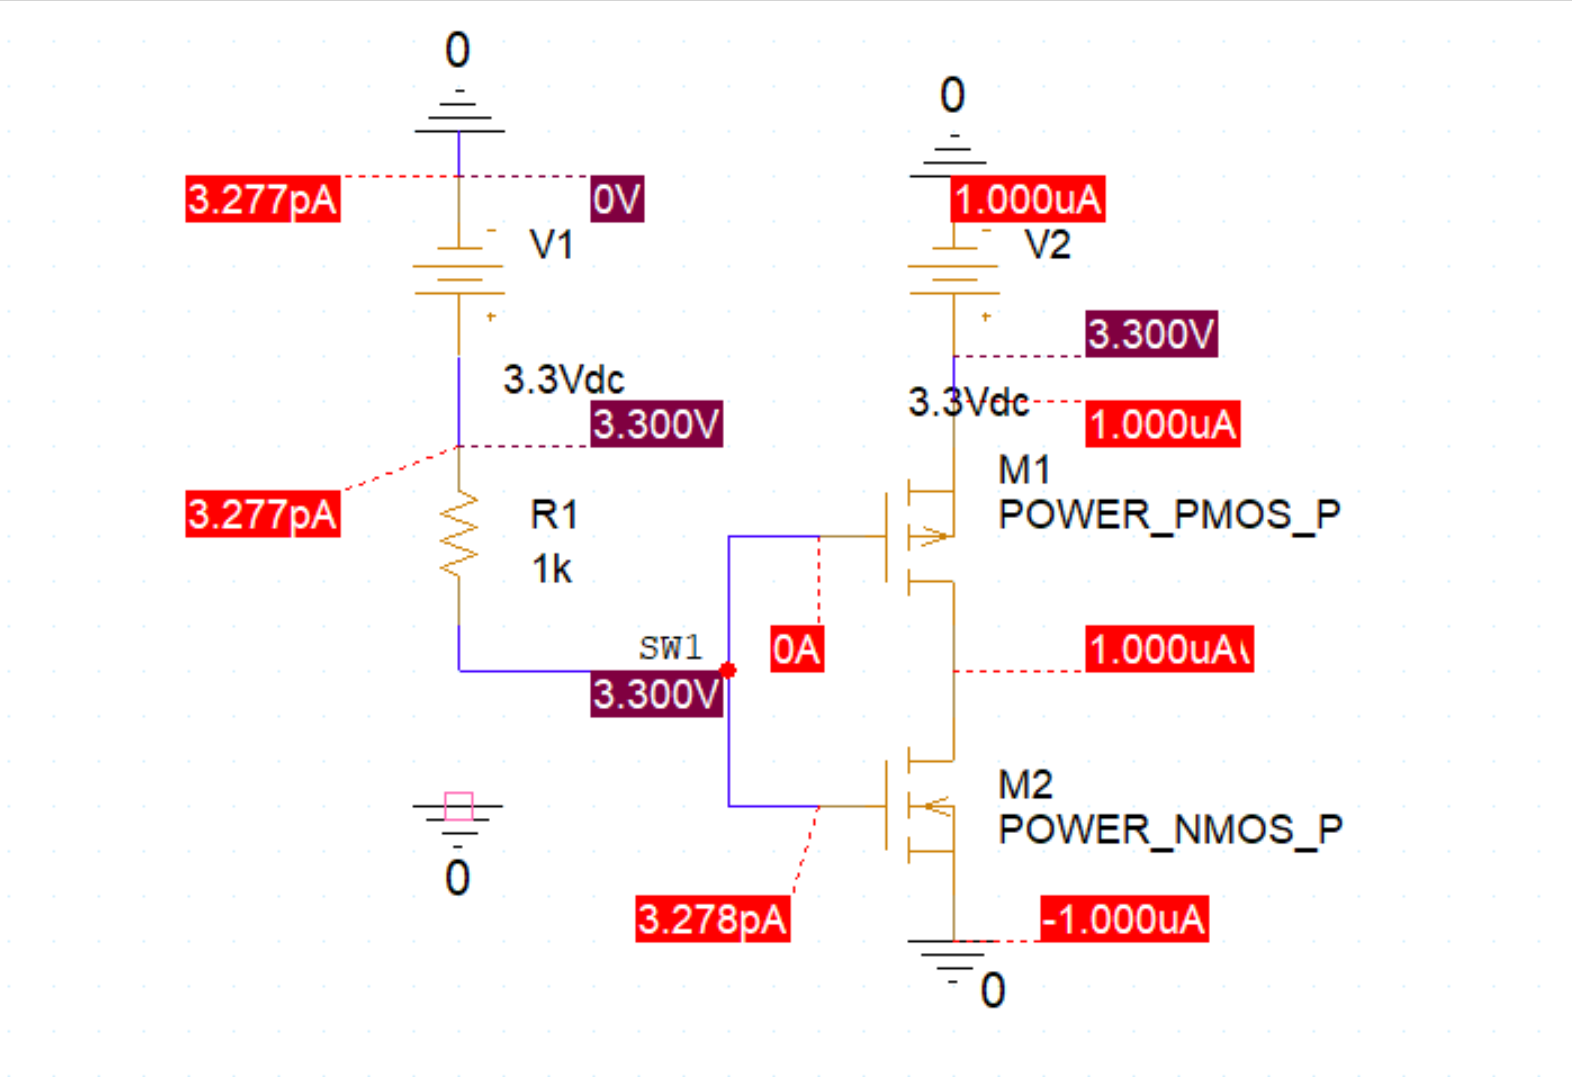
\includegraphics[width=0.7\textwidth]{graphics/section5/f2.png}
    \caption{SW1 OFF}
\end{figure}

\pagebreak
\subsection{Câu 3}
\textbf{Câu hỏi: Trong hình 1.5, điện áp ở đầu ADC1\_CH7 và ADC1\_CH6 là bao nhiêu ?}
\textbf{Trả lời:}

\textit{Xét U3B:}
\begin{itemize}
    \item $V_{out} = V_{in} = 3.3V \cdot \frac{R_8}{R_5 + R_8} = 3.3V \cdot \frac{1k\Omega}{1k\Omega + 1k\Omega} = 1.65V$
    \item Do $R_4, R_9, R_{11}, R_{14}$ mắc nối tiếp với nhau nên: \[I_{R_{14}} = I_{R_4} = \frac{(3.3 / 2) V}{R_4 + R_9 + R_{11} + R_{14}} = \frac{(3.3 / 2) V}{1k\Omega + 100\Omega + 1k\Omega + 1k\Omega} = 532.3 \mu A \]
    \item $V_{ADC1\_CH7} = V_{out} - I_{R_4}.R_4 = 1.65V  - 532.3 \mu A \cdot 1k\Omega = 1.6447V$
\end{itemize}
\textit{Xét U3A:}
\begin{itemize}
    \item $V_{in} = I_{R_{14}}.R_{14} = 532.3 \mu A \cdot 1k\Omega = 532.3mV$
    \item $\beta = \frac{R_{15}}{R_{15} + R_{16}} = \frac{1k\Omega}{1k\Omega + 1k\Omega} = 0.5$
    \item $V_{ADC1\_CH6} = V_{out} \approx V_{in} \cdot \frac{1}{\beta} = 532.3mV \cdot \frac{1}{0.5} = 1064.6mV$
\end{itemize}
\pagebreak
\subsection{Câu 4}
\textbf{Câu hỏi: Trong \ref{subsec:Current sensor circuit}, chúng ta đã áp dụng bộ lọc thông áp (low pass filter) cho tín hiệu ADC\_IN. Tần số cắt (the cutoff frequency) của bộ lọc thông thấp này là gì? Nếu chúng ta muốn đặt tần số cắt là khoảng 10kHz, thì
chúng ta có nên thay đổi những gì trong mạch của U3A?}

\textbf{Trả lời}

Bộ lọc thông áp (low pass filter) là bộ lọc cung cấp đầu ra không đổi từ 0 (DC) đến tần số cắt $f_{OH}$ (the cutoff frequency) và khi lớn hơn $f_{OH}$ sẽ
không truyền tín hiệu nào trên tần số đó.
\[f_{OH} = \dfrac{1}{2\pi RC}\]

Trong mạch \ref{subsec:Current sensor circuit}, ta thấy R = R9 = 1K và C = C10 = 100pF.
\[f_{OH} = \dfrac{1}{2\pi R9.C10} = \dfrac{1}{2\pi .1000.100.10^{-12}} \approx 1,5915 (MHz)\]

Để đạt được tần số cắt khoảng 10kHz, ta phải thay đổi giá trị của R9 và C10 trong mạch của U3A sao cho $ f_{OH} = \dfrac{1}{2\pi.R9.C10 = 10.10^3 Hz}$ hay $ R9.C10 = \dfrac{1}{2\pi.10^4}$
\pagebreak
\subsection{Câu 5}
 \textbf{Câu hỏi: Dòng điện đi qua mỗi LED trong hình 1.7 là bao nhiêu? Ta có thể làm gì nếu ta muốn điều khiển một LED công suất 100mW?}
\textbf{Trả lời:}
\begin{itemize}
    \item Tính toán dòng qua mỗi LED:
    \begin{itemize}
        \item Điện áp phân cực thuận $V_f$ của LED đỏ là 2V, của LED xanh lá là 3V.
        \item $V_{CE_{sat}} = 0.2V$.
        \item $I_{RED\_LED} = \frac{3.3V - V_{f_{RED\_LED}} - V_{CE_{Sat}}}{R_{18}} = \frac{3.3V - 2V - 0.2V}{330\Omega} = 3.33mA$.
        \item $I_{GREEN\_LED} = \frac{3.3V - V_{f_{GREEN\_LED}} - V_{CE_{Sat}}}{R_{19}} = \frac{3.3V - 3V - 0.2V}{330\Omega} = 3.03mA$.
    \end{itemize}
    \item Để điều khiển một LED công suất 100mW:
    \begin{itemize}
        \item Cho $V_LED = 2V$.
        \item $I_{LED} = \frac{P_{LED}}{V_{LED}} = \frac{100mW}{2V} = 50mA$.
        \item $R_{LED} = \frac{V_{CC} - V_{LED} - V_{CE_{Sat}}}{I_{LED}} = \frac{3.3V - 2V - 0.2V}{50mA} = 22\Omega$.
        Vậy $R_{18}$ và $R_{19}$ cần có giả trị tối thiểu $22\Omega$ để điều khiển LED công suất 100mW.
    \end{itemize}
\end{itemize}
\pagebreak
\subsection{Câu 6}
\textbf{Câu hỏi: }

\pagebreak
\subsection{Câu 7}
\textbf{Câu hỏi: Sử dụng IC 74HC595 để thiết kế mạch hiển thị giá trị trên 4 Led 7 đoạn}
\subsubsection{Timer}
Timer là một tính năng quan trọng trong vi điều khiển hiện đại. Chúng giúp đo thời gian thực hiện tác vụ, tạo non-blocking code, kiểm soát pin timing và chạy hệ điều hành. Trong bài tập lớn này, chúng ta sẽ tìm hiểu cách sử dụng timer để chớp tắt đèn LED. Sử dụng timer interrupt để quét LED.
\begin{figure}[ht]
    \centering
    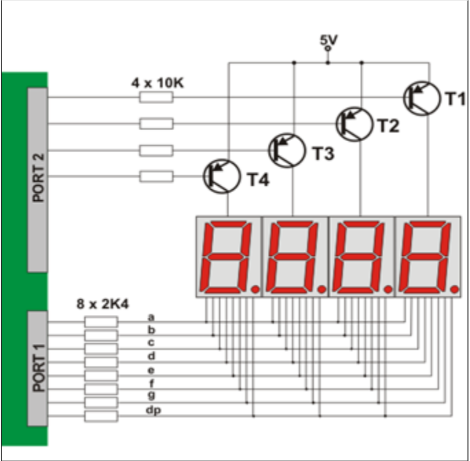
\includegraphics[width=0.7\textwidth]{graphics/LED_7seg.PNG}
    \caption{Giao diện của 4 LED bảy đoạn kết nối với vi điều khiển}
\end{figure}

Mỗi LED bảy đoạn có bảy phân đoạn được đánh dấu từ \textbf{a} đến \textbf{g} \ref{digit} và phân đoạn thứ tám là dấu chấm thập phân. Trong diagram, mỗi LED bảy đoạn có 8 đèn LED bên trong tương ứng với 8 phân đoạn, nên tổng số đèn LED trong ma trận 4 LED bảy đoạn là 32. Tuy nhiên, không cần phải bật tất cả các đèn LED, chỉ cần một trong số chúng. Do đó, chỉ cần 12 chân để điều khiển 4 LED bảy đoạn. Sử dụng vi điều khiển, ta có thể bật các đèn cùng một khoảng thời gian $T_S$. Vì vậy, chu kỳ để  điều khiển 4 LED bảy đoạn sẽ là $4T_S$. Nói cách khác, những LED này được quét với  tần số $f = \frac{1}{4} T_S$. Cuối cùng, dễ thấy nếu tần số quét lớn hơn 30Hz (e.g. f = 50Hz)  thì các LED dường như đang sáng cùng một lúc. Trong bài tập lớn này, timer interrupt được sử dụng để thiết kế một khoảng thời gian $T_S$ cho việc quét LED.
\begin{figure}[ht]
    \centering
    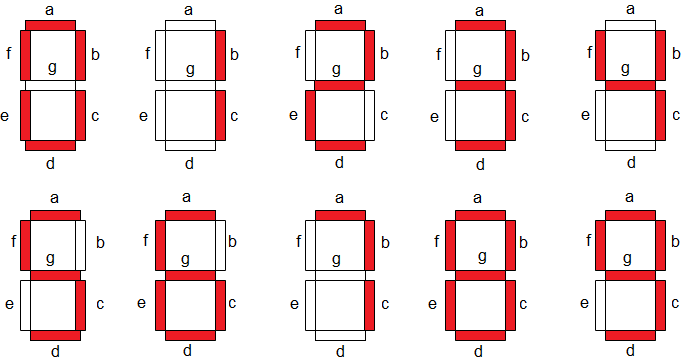
\includegraphics[width=0.7\textwidth]{graphics/digit_Led7.png}
    \caption{Biểu diễn ký tự số bằng LED 7 đoạn}
    \label{digit}
\end{figure}

LED đồng hồ (4 7-segment LEDs) trên kit thí nghiệm không được điều khiển trực tiếp từ chân ESP32. Để tiết kiệm chân, LED đồng hồ được điều khiển thông qua 2 IC 74HC595. IC này có thể giao tiếp với vi điều khiển thông qua giao tiếp SPI.

\subsubsection{Giao tiếp SPI}
\begin{itemize}
    \item SPI - Serial Peripheral Interface - còn gọi là giao diện ngoại vi nối tiếp, chuẩn đồng bộ nối truyền dữ liệu ở chế độ full-duplex (song công toàn phần). Nghĩa là tại 1 thời điểm có thể xảy ra đồng thời quá trình truyền và nhận.
    \item SPI là giao tiếp đồng bộ, bất cứ quá trình nào cũng đều được đồng bộ với xung clock sinh ra bởi thiết bị Master. Do đó, không cần phải lo lắng về tốc độ truyền dữ liệu.
    \item Hoạt động của giao tiếp SPI: sử dụng 4 đường giao tiếp nên đôi khi được gọi là chuẩn truyền thông “ 4 dây”. 4 đường đó là :
    \begin{itemize}
        \item SCK (Serial Clock): Thiết bị Master tạo xung tín hiệu SCK và cung cấp cho Slave. Xung này giữ nhịp cho giao tiếp SPI và truyền dữ liệu. Điều này giúp giảm lỗi và tăng tốc độ truyền.
        \item MISO (Master Input Slave Output): Tín hiệu tạo bởi thiết bị Slave và nhận bởi thiết bị Master. Đường MISO phải được kết nối giữa thiết bị Master và Slave.
        \item MOSI (Master Output Slave Input): Tín hiệu tạo bởi thiết bị Master và nhận bởi thiết bị Slave. Đường MOSI phải được kết nối giữa thiết bị Master và Slave.
        \item CS (Chip Select) hoặc SS(Slave Select): Chọn Slave để giao tiếp. Master kéo chân CS xuống mức 0 (Low) để chọn Slave. Vi điều khiển có thể tạo chân CS bằng cách cấu hình 1 chân GPIO chế độ Output.
    \end{itemize}
\end{itemize}
\begin{figure}[ht]
    \centering
    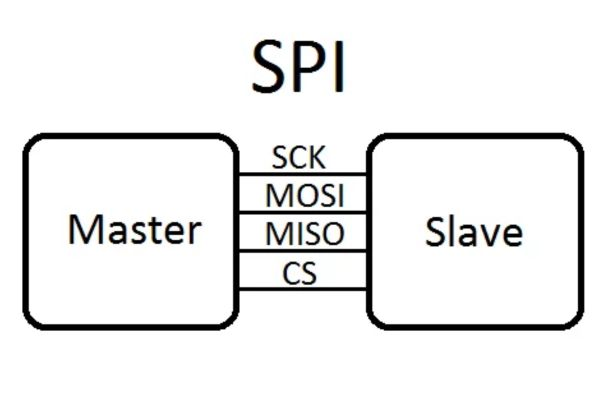
\includegraphics[width=0.5\textwidth]{graphics/spi.jpg}
    \caption{Sơ đồ giao tiếp SPI}
\end{figure}

\subsubsection{IC 74HC595}
74HC595 là một thanh ghi dịch (shift register) hoạt động trên giao thức nối tiếp vào song song ra (Serial IN Parallel OUT), tức là nó có thể nhận dữ liệu đầu vào nối tiếp và điều khiển 8 chân đầu ra song song. Điều này rất tiện dụng khi không có đủ chân GPIO trên vi điều khiển hoặc vi xử lý để kiểm soát số lượng đầu ra cần thiết.

Đối với IC 74HC595, chúng ta cần quan tâm tới các chân SH\_CP, ST\_CP, SDI, SDO, Q0-Q7.

\textbf{Nguyên lý hoạt động:} khi phát hiện cạnh lên tại tín hiệu SH\_CP thì dữ liệu của chân SDI sẽ được đưa vào thanh ghi dịch. Ghi tín hiệu chân ST\_CP xuống mức thấp, thì giá trị trong thanh ghi dịch sẽ được cập nhật ra các chân output Q7->Q0. Để mở rộng thêm tín hiệu output thì ta sẽ dùng 2 IC 74HC595 và kết nối chân SDO của một IC với chân SDI của IC còn lại.

Với 2 IC thì ta có thể điều khiển được 16 output. Để điều khiển LED đồng hồ, ta cần 8 chân để điều khiển tín hiệu LED 7 đoạn, 4 chân để điều khiển chớp tắt 4 LED 7 đoạn, 1 chân để điều khiển dấu hai chấm. Như vậy chúng ta vẫn còn 3 output chưa được sử dụng, 3 output này sẽ được thiết kế để điều khiển LED5, LED6, LED7. Lưu ý: tất cả các chân tín hiệu kể trên đều tích cực mức thấp.

\newpage

Với nguyên lý hoạt động của 74HC595, ta thấy rằng có thể sử dụng SPI để hiện thực giao tiếp giữa MCU và IC. Chân SCK của MCU sẽ kết nối với chân SH\_CP của cả 2 IC, chân MOSI của MCU sẽ kết nối với chân SDI của IC đầu tiên.

\begin{figure}[ht]
    \centering
    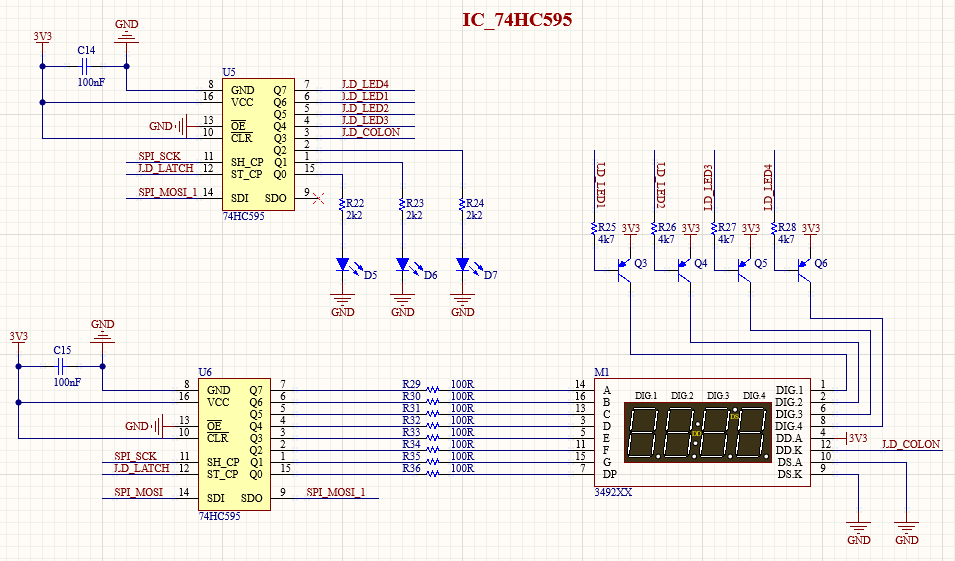
\includegraphics[width=\textwidth]{graphics/sche.PNG}
    \caption{Sơ đồ nguyên lý điều khiển LED đồng hồ}
\end{figure}